\documentclass{article}

\usepackage[english]{babel}
\usepackage[utf8]{inputenc}
\usepackage{amsmath}
\usepackage{graphicx}
\usepackage[breaklinks]{hyperref}
\usepackage[font=footnotesize,labelfont=bf,margin=2.5cm]{caption}
\usepackage{listings}
%\usepackage{subfigure}
\usepackage[round]{natbib}
\bibliographystyle{plainnat}


\title{
	Project 03 \\
	\bigskip
	\normalsize APSC 607 Fall 2017
}

\author{Seth Goodman}

\date{\today}


\begin{document}
\maketitle


%\begin{abstract}
%\end{abstract}

\section{Introduction}
\label{sec:introduction}

This project explores different numerical methods of solving two well-posed initial value problems (IVPs), $y'$, at discrete points within a range $[a\ b]$ for a given initial value $y(a)$ as defined in Equation \ref{eq:intro} and described in \cite{burden2010}. The methods that will be tested are Euler's method (i.e., first order Taylor method), fourth order Runge-Kutta (i.e., essentially fourth order Taylor method), and an implicit trapezoidal method (trapezoidal with Newton Iteration). The behavior and characteristics of these methods will be reviewed and their effectiveness evaluated based on the true solution to the IVP.

\begin{equation}
y' = \frac{dy}{dt} = f(t,y), \qquad a \leq t \leq b, \qquad  y(a) = \alpha
\label{eq:intro}
\end{equation}

All computations are performed using MATLAB using the code accompanying this report. Section \ref{sec:methods} will present the methods used in MATLAB to explore functions. Section \ref{sec:results} contains the results and related outputs for each function, and \ref{sec:conc} includes observations, discussion. All figures and tables found in this report are available in the output subdirectory of the accompanying zip file. Additionally, all code and figures found in the zip file can be accessed via GitHub\footnote{\url{https://github.com/sgoodm/apsc607/tree/master/project_03}}

\newpage
\section{Methods}
\label{sec:methods}

The two unique functions which will be explored in this project, Functions \textbf{A} and \textbf{B}, are defined by Equations \ref{eq:fa} and \ref{eq:fb}, respectively.

\begin{center}
    \centering
    \begin{minipage}{0.5\textwidth}
        \centering
        \begin{equation}
		y' = -9y
		\label{eq:fa}
		\end{equation}
    \end{minipage}\hfill
    \begin{minipage}{0.5\textwidth}
        \centering
        \begin{equation}
        y' = 20 (y-t^2)+2t
		\label{eq:fb}
		\end{equation}
    \end{minipage}
\end{center}


The associated initial values for Functions A and B, are defined by Equations \ref{eq:iva} and \ref{eq:ivb}.


\begin{center}
    \centering
    \begin{minipage}{0.5\textwidth}
        \centering
        \begin{equation}
		y(0) = e
		\label{eq:iva}
		\end{equation}
    \end{minipage}\hfill
    \begin{minipage}{0.5\textwidth}
        \centering
        \begin{equation}
        y(0) = \frac{1}{3}
		\label{eq:ivb}
		\end{equation}
    \end{minipage}
\end{center}


Both IVPs will be examined over the range $ 0 \leq t \leq 1 $, using a baseline step size of $h=0.1$.

To validate and compare each method for solving the IVPs, the true solution is required. The true solution is generated using the Symbolic Toolkit in MATLAB as seen in the example below for Function A.

\bigskip
\begin{lstlisting}[language=Matlab]
	syms y(t)
	ode = diff(y,t) == -9*y;
	cond = y(0) == exp(1);
	sol = dsolve(ode, cond);
\end{lstlisting}
\bigskip


The true values for Functions A and B are compared to the results of integration using the Trapezoidal, Midpoint, and Simpson's Rules for a range of subintervals. The range of subinterval values, \textbf{n}, can vary depending on the function and rule tested, in order to ensure that an accuracy within a tolerance of $10^{-4}$ and $10^{-8}$ of the true value is achieved by at least one \textbf{n} value in the range.

The resulting vector of integral values across varying \textbf{n} can compared with the true integral value generated earlier, to produce an error vector. The error vector is used to identify the value of \textbf{n} (and thus \textbf{h}) at which the integration rule produced results that were accurate within a desired tolerance. No \textbf{n} value needs to be specified for the adaptive approach because, as seen in Subsection \ref{method:adaptive}, this approach iteratively checks (within the function) that a specified tolerance has been reached before producing a single output rather than using a set \textbf{n} value to produce a set of output values.


The remainder of this section will introduce the three composite numerical integration approaches (Trapezoidal, Midpoint, and Simpson's) and the adaptive approach using Simpson's Rule.


\subsection{Euler's (first order Taylor)}
\label{method:euler}

page 266



\subsection{Runge-Kutta Order Four}
\label{method:rk}

page 288



\subsection{Implicit Trapezoidal (Trapezoidal with Newtonian Iteration)}
\label{method:implicit}

page 248



\newpage
\section{Results}
\label{sec:results}

This section will review the results of the different integration rules for Functions A and B. An overview of these results can be seen in Table \ref{table:results}, which shows the the number of subintervals required to reach each tolerance specified, as well as the final error achieved. Figure \ref{fig:true} contains the true plots of both function, for reference.

\bgroup
\footnotesize
\def\arraystretch{1.5}
\begin{center}
	\centering
	\begin{tabular}{l|l|r|r|r}
	\textbf{Function} & \textbf{Method} & \textbf{N: $10^{-4}$} & \textbf{N: $10^{-8}$} &\textbf{Minimum Error} \\
	\hline
	a & trapezoidal & 768  & 65536 & 4.26887e-09 \\
    a & midpoint    & 1024 & 98304 & 8.53747e-09 \\
    a & simpsons    & 42   & 322   & 1.30384e-12 \\
    a & adaptive    & 24   & 278   & -           \\
    b & trapezoidal & 12   & 1082  & 1.29289e-09 \\
    b & midpoint    & 22   & 1522  & 2.58233e-09 \\
    b & simpsons    & 2    & 22    & 2.22044e-16 \\
    b & adaptive    & 2    & 16    & -
	\end{tabular}
	\captionof{table}{Results}
	\label{table:results}
\end{center}
\egroup


% \begin{center}
% 	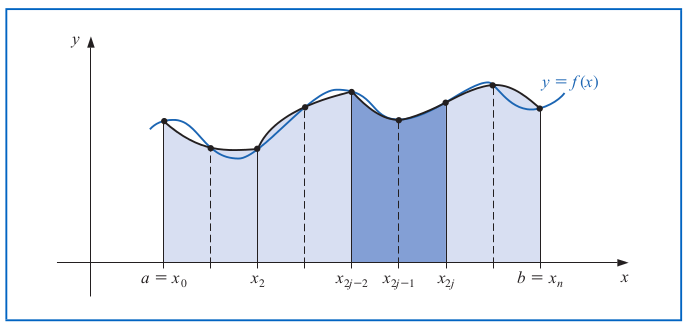
\includegraphics[width=0.9\textwidth]{../additional/simpsons_fig.png}
% 	\captionof{figure}{Simpson's Figure \citep{burden2010}}
% 	\label{sim_fig}
% \end{center}

% \begin{center}
%     \centering
%     \begin{minipage}{0.5\textwidth}
%         \centering
%         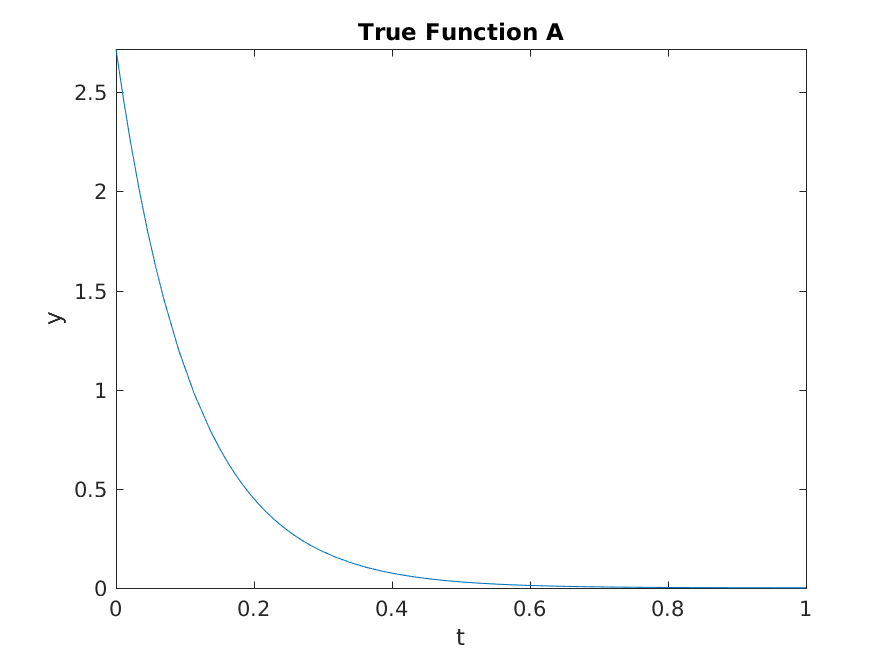
\includegraphics[width=0.99\textwidth]{../output/a_actual.png}
%     \end{minipage}\hfill
%     \begin{minipage}{0.5\textwidth}
%         \centering
%         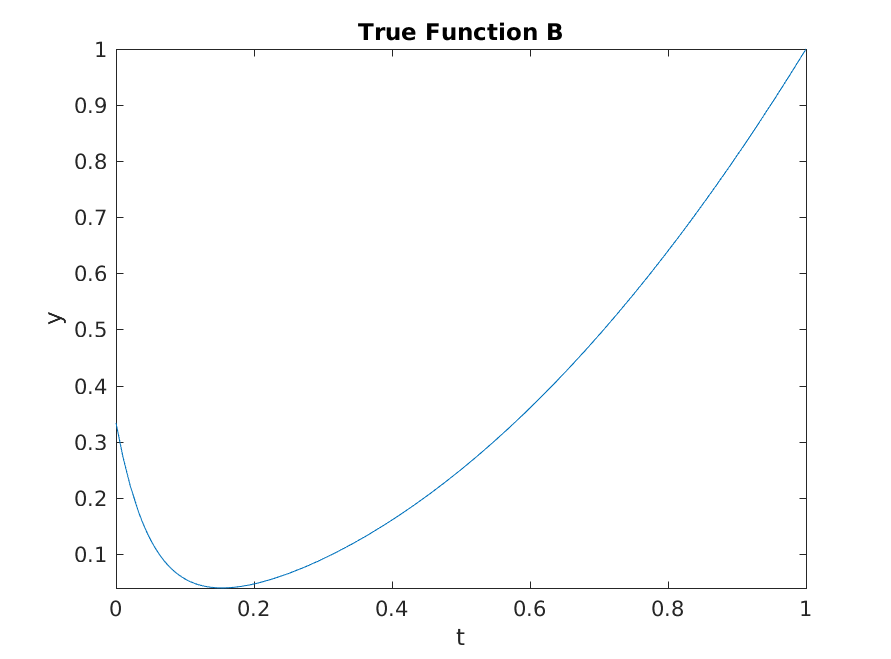
\includegraphics[width=0.99\textwidth]{../output/b_actual.png}
%     \end{minipage}
%   	\captionof{figure}{True plots of Function A and B between zero and two}
% 	\label{fig:true}

% \end{center}


\subsection{Euler's Results}
\label{results:euler}


\subsection{Runge-Kutta Results}\label{results:rk}


\subsection{Implicit Trapezoidal Results}\label{results:implicit}


\section{Discussion and Conclusions}
\label{conc}



\newpage

\bibliography{report}


\end{document}
